% ============================================== %
% Author: Simone Bianco
%
% Thesis Title: IDK something about proofs and circuits and protocols and P $\neq$ NP?
% 
% Bachelor of Science in Computer Science, Sapienza University of Rome.
%
% https://github.com/Exyss/bsc-thesis/
%
% ============================================== %

% Document Class
\documentclass[binding=0.6cm]{sapthesis}

% Packages
\usepackage{microtype}
\usepackage[english]{babel}
\usepackage[utf8]{inputenc}
\usepackage{hyperref}
\usepackage{listings}
\usepackage{xcolor}
\usepackage{xspace}
\usepackage{geometry} 
\usepackage{caption}  
\usepackage[edges]{forest}
\usepackage{subcaption}
\usepackage{float}    
\usepackage{lipsum}  
\usepackage{xargs}                     
\usepackage{booktabs}
\usepackage{graphicx}
\usepackage{makecell}
\usepackage{booktabs}
\usepackage{tabularx}
\usepackage{longtable}
\usepackage{threeparttable}
\usepackage{amsthm}
\usepackage{amssymb}
\usepackage{cleveref}
\usepackage[colorinlistoftodos,prependcaption,textsize=tiny]{todonotes}

\usepackage[
  backend=biber,
  style=alphabetic,
  sorting=anyt,
  minnames=3,
  minalphanames=3
]{biblatex}

% Commands and Settings
\newcommandx{\unsure}[2][1=]{\todo[linecolor=red,backgroundcolor=red!25,bordercolor=red,#1]{#2}}
\newcommandx{\change}[2][1=]{\todo[linecolor=blue,backgroundcolor=blue!25,bordercolor=blue,#1]{#2}}
\newcommandx{\info}[2][1=]{\todo[linecolor=OliveGreen,backgroundcolor=OliveGreen!25,bordercolor=OliveGreen,#1]{#2}}
\newcommandx{\improvement}[2][1=]{\todo[linecolor=Plum,backgroundcolor=Plum!25,bordercolor=Plum,#1]{#2}}
\newcommandx{\thiswillnotshow}[2][1=]{\todo[disable,#1]{#2}}
\newcolumntype{L}[1]{>{\raggedright\arraybackslash}p{#1}}
\newcounter{boxlblcounter}  
\newcommand{\makeboxlabel}[1]{\fbox{#1.}\hfill}
\newenvironment{boxlabel}
  {\begin{list}
    {\arabic{boxlblcounter}}
    {\usecounter{boxlblcounter}
     \setlength{\labelwidth}{3em}
     \setlength{\labelsep}{0em}
     \setlength{\itemsep}{2pt}
     \setlength{\leftmargin}{1.5cm}
     \setlength{\rightmargin}{2cm}
     \setlength{\itemindent}{0em} 
     \let\makelabel=\makeboxlabel
    }
  }
{\end{list}}
\lstdefinestyle{myStyle}{
    belowcaptionskip=1\baselineskip,
    breaklines=true,
    numberstyle=\tiny\color{gray},
    captionpos=b,
    frame=tb,
    basicstyle=\footnotesize\ttfamily,
    keywordstyle=\bfseries\color{green!40!black},
    commentstyle=\itshape\color{blue!40!black},
    identifierstyle=\color{black},
    backgroundcolor=\color{white},
}
\lstset{style=mystyle}

% Metadata
\hypersetup{pdftitle={Thesis},pdfauthor={Simone Bianco}, urlcolor=black, linkcolor=black, colorlinks=true}
\title{IDK something about proofs, search problems, circuits, protocols and P $\neq$ NP?}
\author{Simone Bianco}
\IDnumber{1986936}
\course{Bachelor's Degree in Computer Science}
\courseorganizer{Faculty of Information Engineering, Computer Science and Statistics}
\AcademicYear{2023/2024}
\advisor{Prof. Nicola Galesi\\Prof. Massimo Lauria}
\authoremail{bianco.simone@outlook.it}
\copyyear{2024}
\thesistype{Bachelor's Thesis}

% ================== CUSTOM ENVIRONMENTS ==================

\newtheorem{theorem}{Theorem}
\newtheorem{lemma}{Lemma}
\newtheorem{definition}{Definition}
\newtheorem{claim}{Claim}
\newtheorem{proposition}{Proposition}

% ================== CUSTOM MACROS ==================

\renewcommand{\lnot}{\overline}
\newcommand{\CNF}{\mathsf{CNF}\xspace}
\newcommand{\TFNP}{\mathsf{TFNP}\xspace}
\newcommand{\Search}{\mathsf{Search}\xspace}
\newcommand{\abs}[1]{\left|#1\right|}

% ================== DOCUMENT ==================

\addbibresource{./references.bib}

\begin{document}

\lstset{language=Python}

\frontmatter

\maketitle

% ================== DEDICATION ==================
\dedication{
    Please help me.
}
% ================== ABSTRACT ==================

\begin{abstract}
    Uhhh, idk
\end{abstract}

\let\cleardoublepage\clearpage


\cleardoublepage

\tableofcontents
\let\cleardoublepage\clearpage

\mainmatter

% ================== CHAPTER 1 ==================
\hypersetup{colorlinks=true, linkcolor=blue, citecolor=red}

\chapter{Notes} \label{chap:introduction}

The following definitions and proofs are a reformulation of the results shown in \cite{tfnp_characterization,separations_proof_complexity}

\begin{definition}
    A total query search problem is a sequence of relations $R = \{R_i : R_i \subseteq \{0,1\}^n \times O_i, i \in [n]\}$, where $O_i$ are finite sets called outcome sets, such that $\forall x \in \{0,1\}^n$ there is a $o \in O_i$ for which $(x,o) \in R_n$.

    A total search problem $R$ is in $\TFNP^{dt}$ if its solutions are verifiable through decision trees: for each $o \in O_n$ there is a decision tree $T_o$ with $\mathrm{poly(\log n)}$-depth such that $T_o(x) = 1 \iff (x,i) \in R_n$
\end{definition}

While total search problems are formally defined as sequences $R = \{R_1, \ldots, R_n\}$, it will often make sense to speak of an individual search problem $R_i$ in the sequence. Therefore, we will slightly abuse the notation and also call $R_i$ a total search problem.

\begin{definition}
    Given $R \subseteq \{0,1\}^n \times O$ and $S \subseteq \{0,1\}^m \times O'$, a decision tree reduction from $R$ to $S$ is a set of decision trees $T_i : \{0,1\}^n \to \{0,1\}$ and $T'_o : \{0,1\}^n \to O$, for each $i \in [m]$ and each $o \in O'$, such that
    \[\forall x \in {0,1}^n \;\; ((T_1(x), \ldots, T_m(x)), o) \in S \implies (x, T'_o(x)) \in R\]
\end{definition}

To give an easier intuition of a decision tree reduction, the decision trees $T_i$ map inputs from $Q$ to $R$, while the decision trees $T'_o$ map solutions to $R$ back into solutions of $Q$.

The \textit{size} $s$ of the reduction is the number of input bits to $S$, meaning that $s = m$, while the \textit{depth} $d$ of the reduction is the maximum depth of any tree involved in the reduction
\[d := \max(\{D(T_i) : i \in [m]\} \cup \{D(T'_o) : o \in O_m\})\]

Finally, we define the \textit{complexity} of the reduction as $\log s + d$. Moreover, the denote as $R^{dt}(S)$ the minimum complexity of any decision tree reduction from $R$ to $S$.

Using the previous definition, we can define complexity classes of total query search problems via decision tree reductions. Given a total query search problem $S = (S_n)$, we define the subclass of problems reducible to $S$ as:
\[S^{dt} := \{R : S^{dt}(R) = \mathrm{poly}(\log n)\}\]
where $R = (R_n)$.

Any total query search problem  with solution verifiers $T_o$ for each $o \in O$ can be \textit{encoded} into a canonical unsatisfiable $\CNF$ formula. 

\begin{proposition}
    Given a total query search problem $R \subseteq \{0,1\}^n \times O$, there exists an unsatisfiable $\CNF$ formula $F$ defined on $\abs{O}$-many variables such that $R = \Search(F)$.
    
    This formula is called the canonical $\CNF$ encoding of $R$.
\end{proposition}

\begin{proof}
    Since $R \in \TFNP^{dt}$, for each $o \in O$ there is a $\mathrm{poly}(\log n)$-depth decision tree $T_o$ that verifies $R$. Then, for each $T_o$, let $C_o$ be the clause obtained by taking the disjunction over the conjunction of the literals along each of the accepting paths in $T_o$, meaning that $C_o$ is a $\mathsf{DNF}$ and, by De Morgan's theorem, that $\lnot{C_o}$ is a $\CNF$.

    Let $F := \bigwedge\limits_{o \in O} \lnot{C_o}$. Since each $R$ is a total search problem, for each input there is a valid output, implying that at least one tree $T_o$ will have an accepting path. Hence, by definition of $C_o$, we get that $\lnot{C_o} = 0$, implying that there will always be a false clause in $F$ and thus that $F$ is an unsatisfiable $\CNF$, concluding that:
    \[(x,o) \in R \iff T_o(x) = 1 \iff \lnot{C_o} = 0 \iff (x,o) \in \Search(F)\]
\end{proof}

This result implies that black-box $\TFNP$ is \textit{exactly} the study of the false clause search problem. Then, instead of studying a total search problem $R$, it's sufficient to study the search problem $\Search(F)$ associated with the canonical $\CNF$ encoding $F$ of $R$.

Given a proof system $P$ and an unsatisfiable $\CNF$ formula $F$, we define the \textit{complexity required by $P$ to prove $F$}, denoted with $P(F)$, as:
\[P(F) := \min(\{\deg(\Pi) + \log \mathrm{size}(\Pi) : \Pi \text{ is a $P$-proof of $F$}\})\]
where $\deg$ is the \textit{degree} of the proof, which is a measure defined by the proof system itself. For example, for the Resolution proof system the degree is defined as the \textit{width} of the proof, which is the maximum number of literals in any clause in $\Pi$.

\begin{definition}
    Given $R \in \TFNP^{dt}$, we say that $R$ \textit{characterizes} and a proof system $P$ (and that $P$ \textit{characterizes} $R$) if it holds that $R^{dt} = \{\Search(F) : P(F) = \mathrm{poly}(\log n)\}$.
\end{definition}


\newpage

Tree-like resolutions for an unsatisfiable $\CNF$ formula are strictly connected to the decision trees that solve its associated search problem. In particular, it can be proven that the smallest tree-like refutation has the exact same structure of the smallest decision tree. 

\begin{lemma} \label{lem:treeres_dt}
    \cite{treelike_res_size}
    Let $F$ be an unsatisfiable $\CNF$ formula. If there is a tree-like refutation of $F$ with structure $T$, there also exists a decision tree with structure $T$ that solves $\Search(F)$
\end{lemma}

\begin{proof}
    We procede by induction on the size $s$ of the refutation of $F$.

    Let $F = C_1 \land \ldots \land C_m$. If $s = 1$, then the refutation is made up of only one step that ends with the empty clause, implying that $\exists i \in [m]$ such that $F = C_i = \bot$. Hence, $\Search(F)$ can be solved by the decision tree made of only one vertex labeled with $i$.

    We now assume that every formula with a tree-like refutation with a structure of size $s$ there exists a decision tree with the same structure that solves the search problem associated with the formula.

    Suppose now that the size $s$ of the refutation is bigger than 1. Let $x$ be the last variable resolved by the refutation and let $T_0$ and $T_1$ be the subtrees of $T$ such that $x$ is the root of $T_0$ and $\lnot{x}$ is the root of $T_1$.

    Consider now the formulas $F{\upharpoonright_{x=0}}$ and $F{\upharpoonright_{x=1}}$, respectively corresponding the formula $F$ with the value $0$ or $1$ assigned to $x$. It's easy to see that the subtrees $T_0$ and $T_1$ are valid refutations of the formulas $F{\upharpoonright_{x=0}}$ and $F{\upharpoonright_{x=1}}$: if $b = 0$, then $x$ evaluates to $0$, otherwise if $b = 1$ then $\lnot{x}$ evaluates to 0.

    Since $T_0$ and $T_1$ have size $s-1$, by inductive hypothesis there exist two decision tree with structure $T_0$ and $T_1$ that solve $\Search(F{\upharpoonright_{x=0}})$ and $\Search(F{\upharpoonright_{x=1}})$.

    Finally, the search problem $\Search(F)$ can be solved by the decision tree that queries $x$ and proceeds with the decision tree $T_b$ based on the value $b \in \{0,1\}$ such that $x = b$.

\end{proof}

\begin{definition}
Given two rooted trees $T$ and $T'$, we say that $T$ is embeddable in $T'$ if there exists a mapping $f : V(T) \to V(T')$ such that, for any vertices $u,v \in V(T)$, if $u$ is a parent of $v$ in $T$ then $f(u)$ is an ancestor of $f(v)$ in $T'$.
\end{definition}

\begin{lemma} \label{lem:dt_treeres}
    \cite{treelike_res_size,search_problems_dt_model}
    Let $F$ be an unsatisfiable $\CNF$ formula. If there is a decision tree with structure $T$ that solves $\Search(F)$, there also exists a tree-like refutation of $F$ with structure $T'$ such that $T'$ is embeddable in $T$.
\end{lemma}

\begin{proof}

    The main idea is to associate inductively, starting from the leaves, a clause to each vertex of $T$ in order to transform $T$ in a tree-like refutation of $F$. In particular, each vertex $v$ gets associated to a clause $C(v)$ such that every input of the decision tree that reaches $v$ falsifies $C(v)$.

    Let $F = C_1 \land \ldots \land C_m$. For all $i \in [m]$, we associate the clause $C_i$ to the leaf of $T$ labeled with $i$. This constitutes our base case.

    Consider now a vertex $v$ that isn't a leaf. Let $x$ be the variable that labels $v$ and let $u_0, u_1$ be the vertices such that the edge $(v, u_0)$ is taken if $x = 0$ and the edge $(v, u_1)$ is taken if $x = 1$.  By induction, assume that $u_0$ and $u_1$ have already been associated with the clauses $C_0$ and $C_1$.

    By way of contradiction, suppose that $C_0$ contains the literal $\lnot{x}$. Then, since in a decision tree each variable can be queried only once in every path, there will always be an input with $x = 0$ that reaches $v$. Since $x = 0$ and since $C_0$ contains $\lnot{x}$, this input would satisfy $C_0$, contradicting the fact that $C_0$ was associated to $u_0$ in a way that it is falsified by every input.

    Thus, the only possibility is that $C_0$ can't contain the literal $\lnot{x}$. Similarly, we can show that $C_1$ cant' contain the literal $x$. This leaves us with only two possibilities: either $C_0 = x \lor \alpha$ and $C_1 = \lnot{x} \lor \beta$ or one of $C_0, C_1$ doesn't contain $x, \lnot{x}$.

    In the first case, we can simply associate to $v$ the clause $C = \alpha \lor \beta$.  In the second case, we associate to $v$ the clause that doesn't contain $x, \lnot{x}$ (chose any of them if both clauses do not contain $x, \lnot{x}$).

    In particular, we notice that the first case directly emulates the resolution rule, while the second case essentially represent "redundant steps". By "skipping" these redundant steps, we can obtain a tree $T'$ that is embeddable in $T$ and that contains only nodes on which the first case was applied. Finally, it's easy to deduce that the root node of $T'$ will always be associated with the empty clause $\bot$, concluding that $T'$ is the structure of a tree-like refutation of $F$.

\end{proof}

\begin{theorem}
Let $F$ be an unsatisfiable $\CNF$ formula. The smallest tree-like refutation of $F$ has size $s$ and depth $d$ if and only if the smallest decision tree solving $\Search(F)$ has size $s$ and depth $d$.
\end{theorem}

\begin{proof}
    Let $s$ and $d$ be the size and depth of the smallest tree-like refutation of $F$. Likewise, let $x$ and $y$ be the size and depth of the smallest decision tree solving $\Search(F)$.

    Then, by \Cref{lem:treeres_dt}, we know that there exists a decision tree that solved $\Search(F)$ with the same structure of the smallest refutation. Let $\alpha$ and $\beta$ be the size and depth of this decision tree. It's easy to see that $s = \alpha \geq x$ and $d = \beta \geq y$.

    Viceversa, by the \Cref{lem:dt_treeres}, we know that there exists a tree-like refutation of $F$ such that its structure is embeddable in the one of the smallest decision tree. Let $\gamma$ and $\beta$ be the size and depth of this tree-like refutation. Since the latter is embedded in the smallest decision tree, it's structure must be smaller or equal. Hence, it's easy to see that $x \geq \gamma \geq s$ and $y \geq \delta \geq d$. Thus, we can conclude that $s = x$ and $d = y$.

\end{proof}

\textbf{Note:} the theorem should be generalizable to each tree and not only for the smallest trees.

\newpage

\begin{figure}[H]
\centering

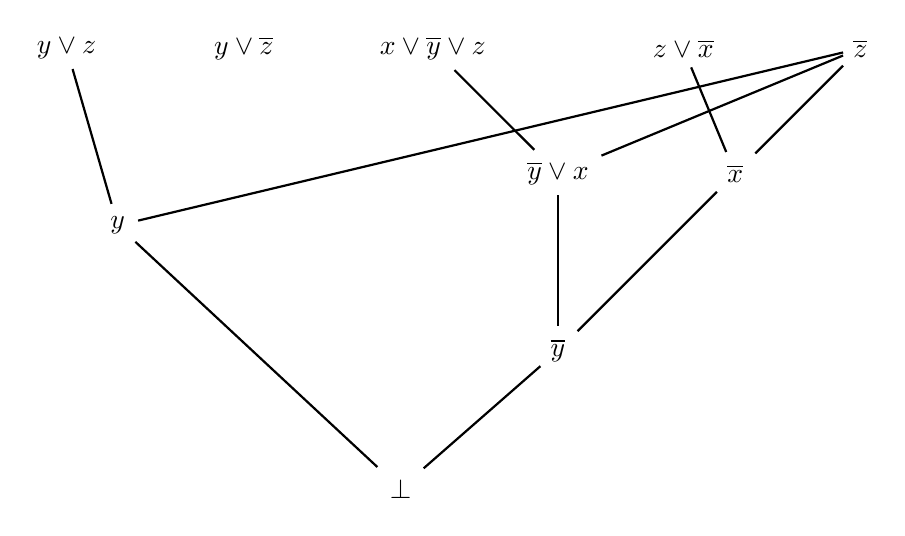
\begin{tikzpicture}[-,>=stealth,shorten >=1pt,auto,node distance=2.25cm, thick,main node/.style={scale=0.9,circle,draw,font=\sffamily\normalsize}]
    \node (1) []{$\bot$};
    
    \node (2) at ($(1)+(-2,1.75)$){};
    \node (3) at ($(1)+(2,1.75)$){$\lnot{y}$};

    \node (4) [above left of=2]{};
    \node (5) [above right of=2]{};

    \node (6) [above of=3]{$\lnot{y} \lor x$};
    \node (7) [right of=6]{$\lnot{x}$};
    
    \node (8) [above left of=6]{$x \lor \lnot{y} \lor z$};
    \node (9) [above right of=6]{$z \lor \lnot{x}$};

    \node (11) [right of=9]{$\lnot{z}$};
    \node (12) [above left of=2]{$y$};

    \node (14) at ($(8)+(-2.4,0)$){$y \lor \lnot{z}$};
    \node (15) [left of=14]{$y \lor z$};

    \path[every node/.style={font=\sffamily\small}]
        (15) edge (12)
        
        (6) edge (3)
        (7) edge (3)
        
        (8) edge (6)
        (11) edge (6)
        
        (9) edge (7)
        (11) edge (7)

        (11) edge (12)

        (12) edge (1)
        (3) edge (1)
    ;
\end{tikzpicture}

\caption{Dag-like refutation of the previous formula}
\end{figure}

\begin{figure}[H]
\centering

\begin{tikzpicture}[-,>=stealth,shorten >=1pt,auto,node distance=2.25cm, thick,main node/.style={scale=0.9,circle,draw,font=\sffamily\normalsize}]

    \node (1) []{$\bot$};
    
    \node (2) at ($(1)+(-2,1.75)$){$y$};
    \node (3) at ($(1)+(2,1.75)$){$\lnot{y}$};

    \node (4) [above left of=2]{};
    \node (5) [above right of=2]{};

    \node (6) [above of=3]{$\lnot{y} \lor z$};
    
    \node (8) [above left of=6]{$x \lor \lnot{y} \lor z$};
    \node (9) [above right of=6]{$z \lor \lnot{x}$};

    \node (11) [right of=9]{$\lnot{z}$};

    \node (14) at ($(8)+(-2.4,0)$){$y \lor \lnot{z}$};
    \node (15) [left of=14]{$y \lor z$};

    \path[every node/.style={font=\sffamily\small}]
        (14) edge (2)
        (15) edge (2)

        (8) edge (6)
        (9) edge (6)

        (6) edge (3)
        (11) edge (3)

        (2) edge (1)
        (3) edge (1)
    ;
\end{tikzpicture}

\caption{Tree-like refutation of the previous formula}
\end{figure}

\begin{figure}[H]
\centering

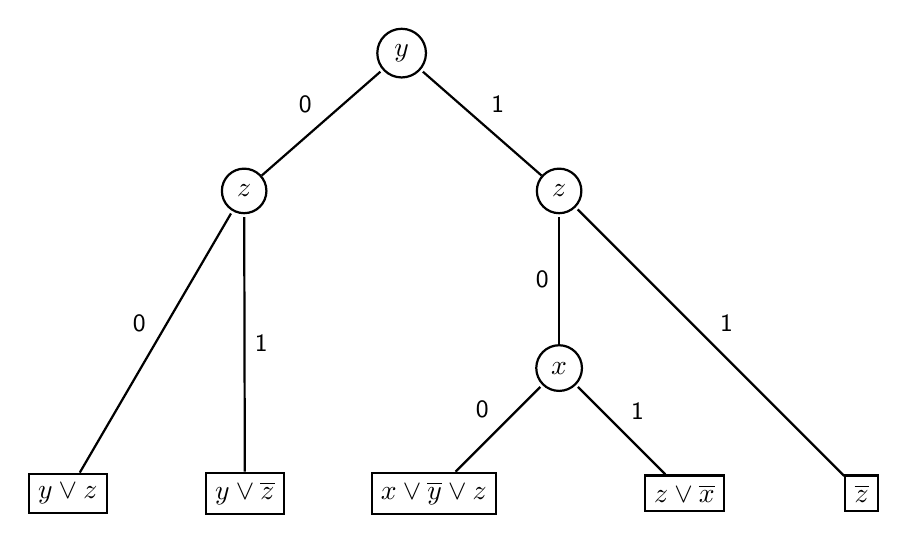
\begin{tikzpicture}[-,>=stealth,shorten >=1pt,auto,node distance=2.25cm, thick,main node/.style={scale=0.9,circle,draw,font=\sffamily\normalsize}]

    \node (1)[circle, draw]{$y$};
    
    \node (2) at ($(1)+(-2,-1.75)$) [circle, draw]{$z$};
    \node (3) at ($(1)+(2,-1.75)$) [circle, draw]{$z$};

    \node (4) [below left of=2]{};
    \node (5) [below right of=2]{};

    \node (6) [below of=3, circle, draw]{$x$};
    
    \node (8) [below left of=6, rectangle, draw]{$x \lor \lnot{y} \lor z$};
    \node (9) [below right of=6, rectangle, draw]{$z \lor \lnot{x}$};

    \node (11) [right of=9, rectangle, draw]{$\lnot{z}$};

    \node (14) at ($(8)+(-2.4,0)$) [rectangle, draw]{$y \lor \lnot{z}$};
    \node (15) [left of=14, rectangle, draw]{$y \lor z$};

    \path[every node/.style={font=\sffamily\small}]
        (14) edge [swap] node{1} (2)
        (15) edge node{0} (2)

        (8) edge node{0}(6)
        (9) edge node[swap]{1}(6)

        (6) edge node{0}(3)
        (11) edge [swap] node{1}(3)

        (2) edge node {0} (1)
        (3) edge node [swap] {1} (1)
    ;
\end{tikzpicture}

\caption{Decision tree for the previous formula}
\end{figure}

\cleardoublepage

% ================== ACKNOWLEDGMENTS ==================
\chapter*{Acknowledgements}

\addcontentsline{toc}{chapter}{Acknowledgements}

No idea

\backmatter
\phantomsection

% ================== BIBLIOGRAPHY ==================
\addcontentsline{toc}{chapter}{Bibliography}
% \bibliographystyle{sapthesis}
% \bibliography{./references.bib}
\printbibliography

\end{document}